\section{Styrhandske}
\begin{figure}[H]
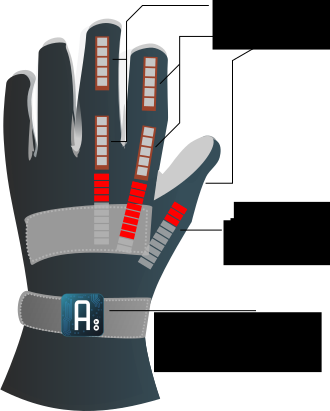
\includegraphics[height=0.5\textheight]{img/kontrollhandske}
\caption{Konceptskiss över styrhandsken.}
\label{kontrollhandske}
\end{figure}
%Detta är intro. Det ska inte vara några detaljer här, bara översiktligt!
% Konvention: styrhandske, inte reglerhandske eller kontrollhanske

För att intuitivt reglera robothanden används en tunn handske som användaren bär på sin hand. På handskens tumme, långfinger och pekfinger finns det två flexsensorer vardera, se figur \ref{kontrollhandske}, som följer användarens hand och ändrar resistans beroende på hur mycket de böjs. På handsken sitter det även tre ledramper som indikerar hur hårt man påverkar objektet. Det tänds fler ledlampor ju större trycket på trycksensorerna är. För att strömförsörja Arduinon, bluetoothmodulen och ledramperna används ett powerpack på 5 Volt, se referenslista \ref{chp:komponentlista}. \comment{borttaget: Resistansen samplas av en mikrokontroller, som efter filtrering trådlöst sänder styrsignaler till robothanden.
Robothanden sänder i sin tur trycket från dess fingrar till styrhandsken. Trycket återkopplas till användaren genom att fler ledlampor på handen tänds ju större trycket är.}


\comment{Emil: Skriv om handens fysiska konstruktion}

\comment{öjeling: fin bild hur signaler åker runt}

\comment{Kanske något enkelet schema för hur det är uppkopplat}




